%!TEX root = ../thesis.tex
\section{オフィスロボットのロボットアームとして要求される項目}
前節で設定した作業(机の片づけ)から導かれる要求事項と,既存オフィスロボットのロボットアーム調査の結果を踏まえて,以下の項目を要求仕様として設定した.なお,QDD モータの使用とオープンプラットフォーム性は,本研究の前提であるため,ここではその他の項目を示す.以下の項目を仕様として,ロボットアームのメカニズム設計を行う.
\begin{itemize}
  \item 0.65m - 0.70mのアームリーチ
  \item 500g以上の可搬重量
  \item 6自由度アーム
  \item 平行グリッパのエンドエフェクタ
\end{itemize}
以下では,これらの項目の詳細について述べる.

\subsection{アームリーチ}
前節で設定した作業より,ロボットアームから0.5m以内の範囲にある対象物を扱えることが要求される.また,既存のオフィスロボット 10 台のアームリーチを調査した結果(図\ref{fig:reach}参照),最小は0.51m,最大は0.90mで,平均値および中央値はいずれも0.71mであった.そこで,本研究ではアームリーチを0.65mから0.70mの範囲に設定した.
\begin{figure}[h]
  \centering
  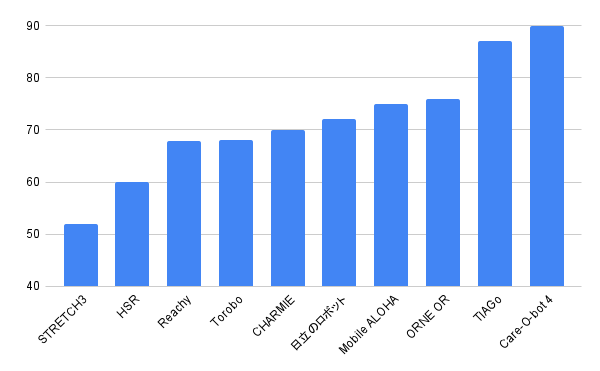
\includegraphics[width=10cm]{images/2syou/reach.png}
  \caption{Office robot arm reach survey results}
  \label{fig:reach}
\end{figure}

\subsection{可搬重量}
机の片づけ作業では,最大500gの物体の把持が求められる.また,既存ロボットアーム調査では,可搬重量の最小は0.35kgであった(図\ref{fig:payload}参照).よって,現時点のオフィス作業においては0.5kg以上の可搬重量を確保できれば十分であると考えられるため,本研究では0.5kg以上を可搬重量の要件とした.
\begin{figure}
  \centering
  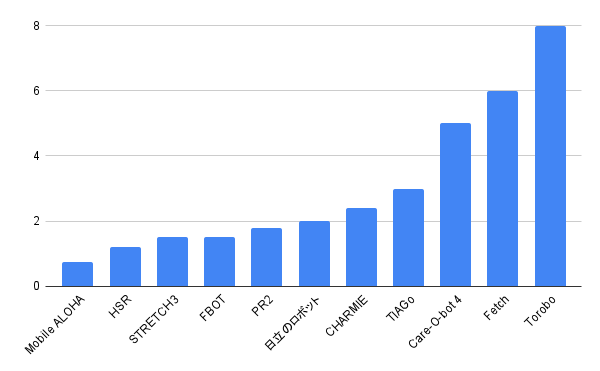
\includegraphics[width=10cm]{images/2syou/payload.png}
  \caption{Office robot payload survey results}
  \label{fig:payload}
\end{figure}
\clearpage

\subsection{自由度}
既存のオフィスロボットのアームの自由度を調査したところ,6自由度と7自由度のロボットが大半であった(\ref{fig:armDof}参照).6自由度の軸配置は,肩2軸(ピッチ,ロール),肘1軸(ロール),手首3軸(ロール,ピッチ,ヨー)で,7自由度ロボットは肩にロール軸が追加されている.7自由度アームは6自由度アームに比べて姿勢の自由度が増す一方で,アーム重量やコストが増加する.本研究ではコスト削減と軽量化を優先し,6自由度を採用した.
\begin{figure}[h]
  \centering
  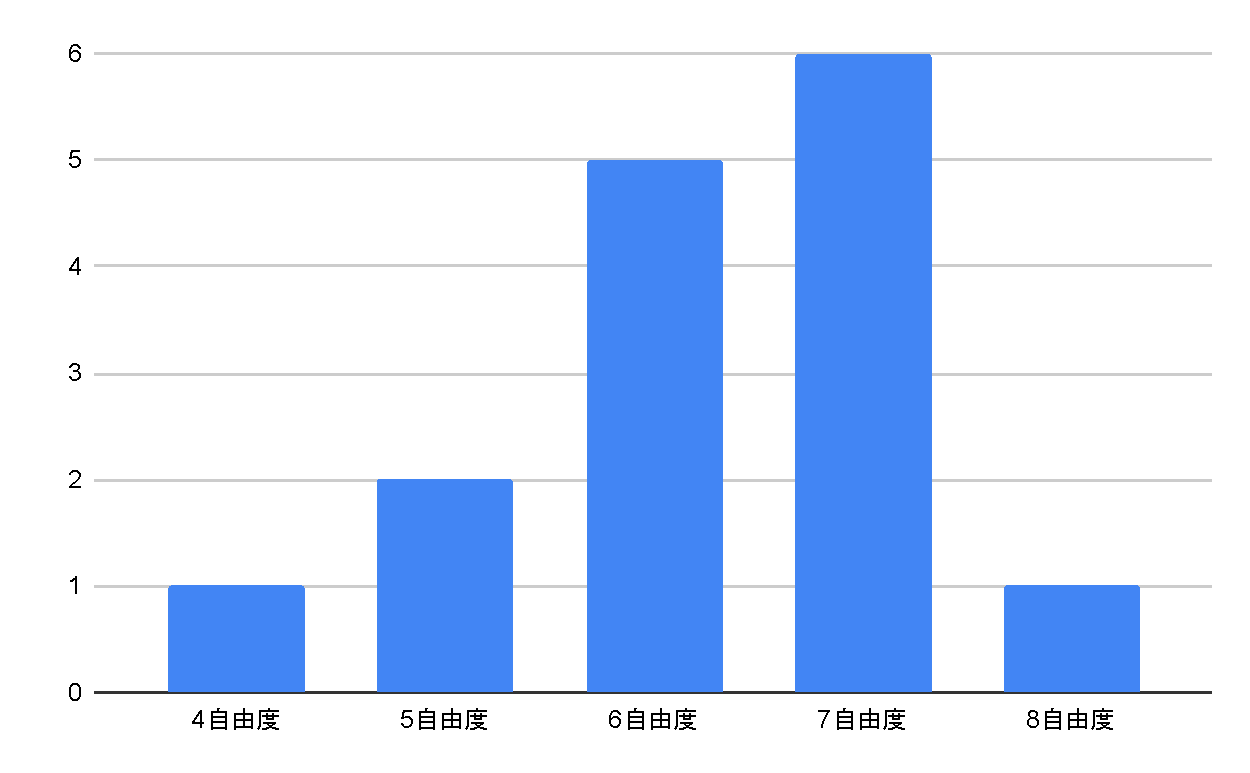
\includegraphics[width=10cm]{images/2syou/armDof.pdf}
  \caption{Office robot arm DoF survey results}
  \label{fig:armDof}
\end{figure}
\clearpage

\subsection{エンドエフェクタの形状}
既存のオフィスロボットで多く採用されているエンドエフェクタは,TIAGoのような平行グリッパ(図\ref{fig:tiago_hand}参照)である.TIAGoを開発しているPAL Robotics社が公開している動画\cite{TIAGo-movie:online}では,布,ジュース缶,スプレー缶,ジュースパック,板状物など多様な形状の物体を把持している様子が確認できる.本研究においても多様な形状の物体把持が求められるため,平行グリッパを採用した.
\begin{figure}[h]
  \centering
  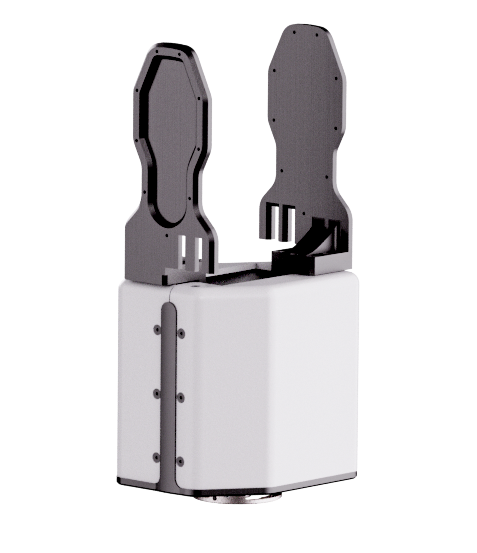
\includegraphics[width=8cm]{images/2syou/tiago_hand.png}
  \caption{End effectior of TIAGo}
  \label{fig:tiago_hand}
\end{figure}
\clearpage
\newpage